\documentclass[letterpaper]{article}
\usepackage[utf8]{inputenc}
%\usepackage[latin1]{inputenc}
\usepackage[spanish]{babel}
\usepackage{geometry}
\usepackage{anysize}
\usepackage{graphicx} 
\usepackage{amsmath}
%\numberwithin{equation}{list}
\marginsize{1cm}{2cm}{0cm}{2cm}  
\title{Tarea Examen - Ecuaciones diferenciales ordinarias \\ \begin{large}Curso de Física Computacional\end{large}}
\author{M. en C. Gustavo Contreras Mayén}
\date{ }
\begin{document}
\maketitle
\fontsize{14}{14}\selectfont
\spanishdecimal{.}
\begin{enumerate}
\item Se dispara un proyectil al aire con un ángulo de $45^{\circ}$ con respecto al suelo, con $u=v=150 m/s$, donde $u$ y $v$ son las velocidades horizontal y vertical, respectivamente. Las ecuaciones de movimiento están dadas por
\begin{eqnarray*}
u^{'} & = & -c Vu, \hspace{1.5cm} u(0)=150 m/s \\
v^{'} & = & -g - cVv, \hspace{1.5cm} v(0)=150 m/s
\end{eqnarray*}
donde $u$ y $v$ son funciones del tiempo, $u=u(t)$ $y v=v(t)$ y
\begin{eqnarray*}
V & = & \sqrt{u^{2} + v^{2}} \\
c & = & 0.005 \hspace{2cm} \text{(coeficiente de arrastre)} \\
g & = & 9.9 m/s^{2}
\end{eqnarray*}
Las ecuaciones de movimiento se pueden resolver mediante alguno de los métodos de Runge-Kutta. La trayectoria del proyectil se puede determinar al integrar
\[ x' = u \hspace{2cm} \text{y} \hspace{2cm} y' = v \]
o bien
\begin{eqnarray*}
x & = & \int^{t}_{0} u(t') dt' \\
y & = & \int^{t}_{0} v(t') dt'
\end{eqnarray*}
\begin{enumerate}
\item Escribe un programa en Fortran con el método RK2 que resuelva y grafique la trayectoria del proyectil.
\item Re-escribe el programa, ahora con el metodo RK3 (compara la gr\'{a}fica contra la obtenida del inciso anterior).
\end{enumerate}
\item Un tubo en forma de U y $0.05$ m de radio se llena con agua, pero con una división de forma que el nivel del agua en la parte vertical de la izquierda es $0.2$ cm más alto que el de la parte vertical derecha. En el instante $t=0$ se retira la división. El nivel del agua de la parte izquierda $y_{a}A$, medido desde el plano intermedio entre las dos superficies, satisface la ecuación
\[ Ly_{a}^{''} = -2 gy_{a} \]
donde $L$ es la longitud total del agua en el tubo, que mide $1$ m. Si se desprecia la fricción del tubo, calcula el nivel del agua por medio del método de Euler haica adelante para $0 < t < 10$ s y determina cuándo alcanza $y_{a}$ su máximo y su mínimo. Utiliza $h=0.001$.
\item Repite el problema anterior, pero ahora suponiendo que hay fricción en el tubo de forma que la ecuación de movimiento es 
\[ Ly_{a}^{''} = -2 gy_{a} - \beta y_{a}{'}\]
donde $\beta=0.8$ m/s. Usa nuevamente $h=0.001$.
\item Un depósito cónico contiene agua hasta $0.5$ m de altura a partir del fondo. el depósito tiene un orificio en el fondo, de $0.02$ m de radio. El radio del depósito está dado por $r=0.25y$, donde $r$ es el radio y $y$ la altura medida desde el fondo. La velocidad del agua que pasa por el orificio está dada por $v^{2}=2gy$. Por medio del método de Euler hacia adelante ($h=0.001$), calcula cuántos minutos se tardará en vaciar el depósito.
\item \begin{enumerate}
\item Un tanque de 50 galones de agua contiene sal con una concentración de 10 onzas/galón. Con el fin de diluir el contenido de sal, se suministra agua pura a razón de 2 galones/minuto. Si el depósito tiene una mezcla uniforme y la misma cantidad de agua que entra sale del depósito cada minuto, la concentración de sal satisface\\
\[ y'_{1}(t)= -\frac{2}{50}y_{1}, \hspace{1.5cm} y_{1}(0)=10 \]\\
donde $y_{1}(t)$ es la concentración de sal en onzas/galón y $t$ es el tiempo en minutos. Usando el método de Runge-Kutta de segundo orden y $h=1$ minuto para determinar cuánto tiempo debe de transcurrir para que la concentración de sal sea $1/10$ de su valor inicial.
\item El agua que sale del tanque entra a otro tanque de 20 galones, en el cual también se vierte agua pura a razón de 3 galones/minuto y se mezcla bien. La concentración de sal en el segundo tanque satisface
\[ y'_{2}(t)= -\frac{3}{20}y_{2}(t)+\dfrac{2}{20}y_{1}(t), \hspace{1.5cm} y_{2}(0)=0 \]
donde $y_{1}(t)$ es la concentración de sal del tanque de 50 galones del problema anterior. Usando RK2, determina cuándo alcanza su máximo de concentración de sal en el tanque de 20 galones. Supongamos que el segundo tanque tiene agua pura en $t=0$.
\end{enumerate}
\item Calcula $y(2)$ para la siguiente ecuación por medio de RK2, con $h=1$
\[ y^{''} +0.2 y{'} + 0.003 y \sin(t) = 0, \hspace{1cm} y(0)=0, y{'}(0)=1 \]
\item Repite el problema anterior, ahora con el método RK3
\item La corriente eléctrica de un circuito $RLC$ en serie, satisface la ecuación\\
\[ L \frac{di}{dt}+ Ri+ \frac{1}{C} \int_{0}^{t} i(t') dt' +\frac{1}{C}q(0)= E(t), \hspace{1.5cm} t>0 \]\\
cuando el circuito se cierra en el instante $t=0$, se tiene que $i=i(t)$ es la corriente, R es la resistencia, $L,C,E$ vienen dadas por: $L=200H$, $C=0.001F$, $E(t)=1V$ para $t>0$.\\
Las condiciones iniciales son $q(0)=0$ (carga inicial del condensador), $i(0)=0$. Calcular la corriente para $0 \leq t \leq 5$ segundos y el factor de amortiguamiento y la frecuencia de oscilación del circuito $RLC$ para los siguientes valores de R:\\
\begin{enumerate}
\item $R = 0 \hspace{0.1cm} \Omega$
\item $R = 50 \hspace{0.1cm} \Omega$
\item $R = 100 \hspace{0.1cm} \Omega$
\item $R = 300 \hspace{0.1cm} \Omega$
\end{enumerate}
Discute de acuerdo con al teoría de electricidad qué es lo que sucede con cada uno de los casos en donde se varía el valor de la resistencia $R$.
\item El movimiento del sistema de masas que se muestra en la figura (1) está dado por:
\[ y'' + 2 \zeta \omega y' + \omega^{2}y = \dfrac{F(t)}{M}\]
donde \\ 
$\omega = \left( \dfrac{k}{M} \right)^{2}$ (frecuencia natural sin amortiguamiento, $s^{-1}$) \\
$\zeta = \dfrac{c}{2M\omega}=0.5$ (factor de amortiguamiento) \\
$k = 3.2$ (constante del resorte, $\frac{kg}{s^{2}}$ \\
$M=5$ (masa, kg) \\
$F(t) = 0$ (fuerza, Newtons)
\begin{figure}[!h]
	\centering
	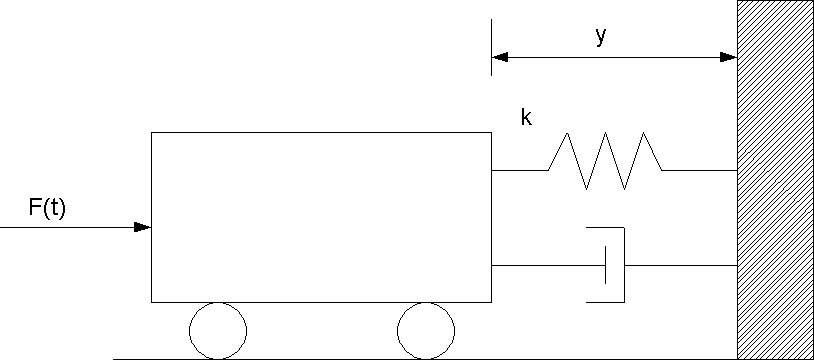
\includegraphics[scale=0.4]{Figura01.png}  
	\label{fig:figura01}
	\caption{Sistema masa-resorte.}
\end{figure}
\\Si $F(t)$ es una función escalonada de magnitud $F_{0}=1$ kg y cuya duración es 1 segundo, determina el movimiento de la masa para $0<t<10$ segundos por medio del método de Runge-Kutta de cuarto orden.
\item Determina la respuesta y carga dinámica del sistema amortiguado del problema anterior sujeto a un pulso de fuerza triangular
\begin{equation*}
F(t) =
	\begin{cases}
2F_{0}t,  & 0 \leq t \leq 1 s\\
2F_{0}(1-t), & 1 \leq t \leq 2 s\\
0, & t>2 s
\end{cases}
\end{equation*}
Donde $F_{0}=1$ Kg (fuerza). Utiliza el método RK4.
\end{enumerate}
\end{document}